\chapter{TINJAUAN PUSTAKA}
\label{chap:tinjauanpustaka}

% Ubah bagian-bagian berikut dengan isi dari tinjauan pustaka

\section{Penelitian Terkait}
\label{sec:penelitianterdahulu}
Pada sub bab ini akan disampaikan penelitian terdahulu yang berkaitan dengan penelitian ini.
\subsection{Deteksi Rebar Untuk Mengukur Perbedaan Material Rebar}

Dalam studi yang berjudul "Rebar Detection - POD AApproach to Determine the Reliability of GPR Systems and to Quantify the Influence of Different Material Parameters" \parencite{Feistkorn2016} dipaparkan keefektivitasan dari GPR untuk mengukur pengaruh dari perbedaan parameter material. Pada penelitian ini dijelaskan bahwa pantulan sinyal GPR memiliki hasil keakuratan yang berbeda bergantung dari penyusun beton itu sendiri, termasuk diamter dari rebar dan kondisi dari beton itu sendiri. Penelitian ini memiliki hasil yang baik dengan tingkat akurasi 90\%. Meskipun objek yang diuji adalah rebar, namun pada penelitian ini tidak berfokus pada deteksi rebar itu sendiri.

\subsection{Deteksi Rongga Udara pada Beton Menggunakan Radar dengan Konfigurasi ZOP}

Selain itu terdapat penelitian yang berjudul "Detection of air voids in concrete by radar in transmission mode" \parencite{Trela2015} disampaikan tentang pendeteksian rongga udara yang sangat berbahaya bagi kesehatan beton dan bangunan dalam jangka panjang. Pendeteksian rongga udara dilakukan pada beton buatan dengan konfigurasi ZOP. Penelitian ini memberikan hasil yang cukup baik dimana metode ZOP memiliki potensi dalam deteksi air void.

\subsection{Klasifikasi Jenis Tanah dari GPR B Scan Menggunakan Teknik Deep Learning}

Selain itu terdapat penelitian yang berjudul "Classification of soil types from GPR B Scans using deep learning techniques" \parencite{Barkataki2021} disampaikan tentang pengklasifikasian jenis tanah dimana gelombang sinyal B-Scan didapatkan dari simulasi gprMax. Penelitian ini memberikan hasil yang cukup baik dimana klasifikasi jenis tanah menghasilkan akurasi hingga 97\%.

Dari ketiga penelitian tersebut, terdapat beberapa research gap antara lain: deteksi hanya berfokus ke satu objek saja, deteksi rongga udara dilakukan pada satu variasi bentuk media, dan menggunakan konfigurasi ZOP dari penggunaan radar dan penggunaan gprMax baru untuk sinyal tanah. Hal ini menunjukkan adanya peluang penelitian yang signifikan untuk mengembangkan model CNN yang dapat bekerja dengan data sinyal GPR untuk deteksi airgap atau rongga udara yang lebih akurat dan efisien dalam konteks struktur beton.

\section{Teori/Konsep Dasar}
Pada sub bab ini akan dijelaskan teori yang berkaitan dengan penelitian ini.
\subsection{Rongga Udara}
Rongga udara di beton dapat membahayakan integritas dan daya tahan material. Karena pemadatan yang tidak tepat atau ketidakkonsistenan campuran, rongga ini sering terbentuk pada beton selama proses pengecoran. Hal ini mengganggu konsistensi matriks beton, yang mengurangi kapasitasnya untuk menahan beban dan meningkatkan kerentanannya terhadap retak tekanan. Rongga udara juga dapat memungkinkan uap air dan bahan kimia berbahaya masuk, yang mempercepat korosi tulangan baja yang tertanam dan kerusakan beton. Penetrasi kelembapan ini dapat menyebabkan kerusakan beku-cair di iklim dingin, yang membuat struktur lebih lemah. Jika beton diharapkan dapat menahan beban dinamis atau beban tumbukan, rongga udara mengurangi kemampuan material untuk menyerap dan mendistribusikan gaya\parencite{Zhu2007}.

\subsection{Ground Penetrating Radar}
Ground Penetrating Radar (GPR) atau juga disebut Surface Penetrating Radar (SPR) adalah radar untuk melihat kondisi di bawah tanah. GPR sendiri terdiri dari beberapa bagian inti seperti unit pusat, antena pemancar, antena penerima, dan komputer. Unit pusat memancarkan sinyal elektromagnetik ke tanah oleh antena pemancar. Sinyal dipancarkan ke semua arah, tetapi sebagian besar energi dipancarkan dalam volume kerucut di bawah antena, seperti ditunjukkan pada gambar berikut \parencite{Daniels2004}:

\begin{figure} [H] \centering
  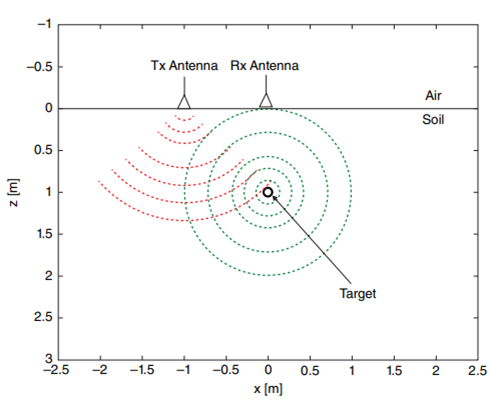
\includegraphics[scale=0.7]{gambar/bab2/gpr1.png}
  \caption{Prinsip kerja GPR \parencite{Persico2014}}
  \label{fig:GPRKerja}
\end{figure}

Ketika gelombang elektromagnetik bertemu dengan objek yang terkubur di dalam tanah, gelombang tersebar ke semua arah sesuai dengan pola tertentu. Pada penerapannya, antena pemancar dan penerima dipasang pada struktur yang kuat menjadi satu. Sinyal yang dikumpulkan biasanya ditampilkan secara real-time di layar komputer3 dan disimpan di hard disk computer. Prinsip kerja GPR tidak jauh berbeda dengan radar pada umumnya. Akan tetapi, terdapat perbedaan dalam hal teknologi, kebutuhan, aplikasi, dan pita frekuensi. GPR harus mengidentifikasi target statis, dan interpretasi data tidak diminta secara real-time. Di sisi lain, dalam prospeksi GPR gelombang elektromagnetik tidak merambat di udara tetapi malah merambat di media inang yang lebih rumit, biasanya berkerugian dan tidak homogen, mungkin dispersif, dan dalam beberapa kasus anisotropik dan/atau magnetik. GPR terbagi menjadi 2 sistem yakni pulsed dan stepped-frequency. Pulsed memancarkan dan menerima gema ke pulsa elektromagnetik. Stepped-frequency mendekomposisi pulsa elektrom agnetik menjadi komponen spektralnya dan memancarkannya secara berurutan. Akibatnya, memancarkan dan menerima kereta sinyal sinusoidal\parencite{Persico2014}.

Mengacu dari terminology data GPR untuk titik ruang disebut A-scan atau jejak GPR.
\begin{figure} [H] \centering
  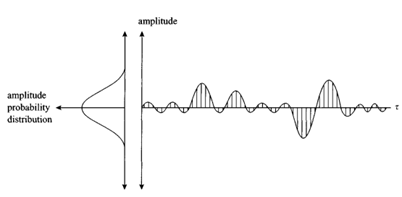
\includegraphics[scale=1]{gambar/bab2/gpr2.png}
  \caption{Sinyal A-scan \parencite{Daniels2004}}
  \label{fig:GPRAscan}
\end{figure}
Kumpulan jejak GPR untuk garis yang dipindai disebut B-scan. Meskipun GPR biasanya mengumpulkan data saat bergerak, model "stop-gather-and-go-on" dianggap cukup akurat dikarenakan perbedaan kecepatan antara sinyal elektromagnetik dan operator manusia. Penyimpanan A-scan bisa memakan waktu lebih lama karena alasan teknis.
\begin{figure} [H] \centering
  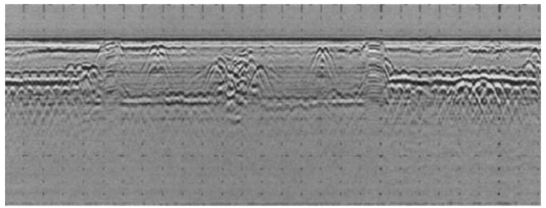
\includegraphics[scale=1]{gambar/bab2/gpr3.png}
  \caption{Sinyal B-scan \parencite{Daniels2004}}
  \label{fig:GPRBscan}
\end{figure}
Namun, menjaga kecepatan konstan saat mengumpulkan data adalah praktik terbaik. Set data GPR dari B-scan paralel disebut C-scan. Yang biasa dilihat di lapangan adalah B-scan. Data awal, atau data mentah, bisa lebih jelas setelah pemrosesan\parencite{Daniels2004}.
\begin{figure} [H] \centering
  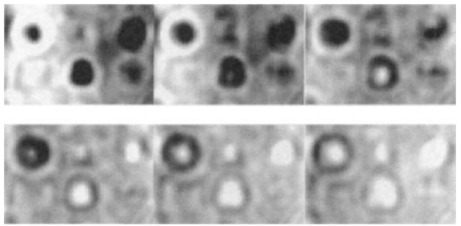
\includegraphics[scale=1]{gambar/bab2/gpr4.png}
  \caption{Sinyal C-scan \parencite{Daniels2004}}
  \label{fig:GPRCscan}
\end{figure}

\subsection{gprMax}
gprMax dikembangkan sebagai perangkat lunak lintas platform untuk Linux, Microsoft Windows, dan kemudian Mac OS X. GprMax ditulis dengan bahasa pemrograman C, dengan bagian yang memerlukan perhitungan intensif - loop solver FDTD - diparalelkan menggunakan OpenMP \parencite{Craig2016}. Pengembangan gprMax dalam implementasi fitur-fitur lanjutan baru dan untuk meletakkan dasar untuk pengembangan masa depan, diputuskan bahwa kode harus ditulis ulang menggunakan bahasa yang berorientasi objek. Python adalah bahasa yang berorientasi objek dan menampilkan pengetikan dinamis dan manajemen memori otomatis. Ini juga dimaksudkan untuk sangat mudah dibaca dan dapat diperluas. Namun, kemudahan dan fleksibilitas Python memiliki beberapa kekurangan salah satunya adalah kecepatan dalam penulisan. Kehilangan kecepatan ini dapat diatasi dengan menggunakan Cython - sebuah superset dari Python yang menghasilkan kode C yang efisien yang dapat dikompilasi menjadi modul ekstensi. Versi baru dari gprMax telah dikembangkan ulang dengan kombinasi Python, NumPy, dan Cython dengan OpenMP, yang mempertahankan manfaat Python dengan kecepatan C yang paling \parencite{Craig2015}.

gprMax menggunakan file input berupa teks di mana pengguna menentukan semua parameter untuk simulasi, misalnya, ukuran model, diskretisasi, jendela waktu, geometri, bahan, dan eksitasi. Penggunaan software gprMax sendiri tidak disertai dengan GUI. GUI tidak dikembangkan karena dinilai terlalu rumit bagi pengguna apabila berurusan dengan banyak nilai parameter yang harus diinputkan dalam satu waktu Berikut adalah contoh file input untuk simulasi GPR 2D sederhana dari silinder logam yang dikubur di setengah ruang dielektrik tanpa kerugian\parencite{Craig2016}.
\begin{figure} [H] \centering
  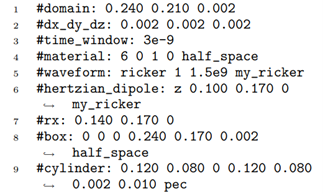
\includegraphics[scale=1]{gambar/bab2/gprmax1.png}
  \caption{Contoh file input simulasi gprMax \parencite{Craig2016}}
  \label{fig:gprMaxSim}
\end{figure}
Disamping itu, gprMax mengandung banyak fitur yang kuat dan dapat disesuaikan untuk pemodelan GPR. Selama 20 tahun terakhir, model antena telah dimasukkan dalam simulasi numerik GPR. Model antena actual telah dimasukkan terutama dari antena yang digunakan di dunia akademik atau untuk tujuan penelitian. Telah ada sedikit pekerjaan yang diterbitkan dari simulasi GPR dengan model antena komersial. Namun, kemajuan dalam kekuatan komputasi, ditambah dengan keinginan untuk menyelidiki informasi amplitudo kuantitatif dari GPR, terdapat kebutuhan untuk mengembangkan dan menggunakan model FDTD 3D rinci dari antena GPR realistis dalam simulas\parencite{Craig2016}.

GprMax2D dan GprMax3D merupakan dua program yang mengimplementasikan metode FDTD untuk pemodelan GPR di 2D dan 3D. Beberapa fiturnya adalah: antarmuka perintah yang mudah digunakan, kemampuan untuk memodelkan bahan dispersif, pemodelan target berbentuk kompleks serta simulasi ruang tak terbatas menggunakan kondisi batas penyerapan yang kuat. GprMax3D mampu mensimulasi antena GPR dan bahkan pengenalan garis transmisi pemberian mereka ke dalam model. GprMax2D digunakan untuk simulasi "signture" GPR sedangkan GprMax3D digunakan untuk simulasi yang lebih detail dan realistis terutama ketika perbandingan dengan data GPR nyata penting. Baik program GprMax2D dan 3D menggunakan file ASCII (teks) sederhana untuk mendefinisikan parameter model \parencite{Giannopoulos2005}.
\begin{figure} [H] \centering
  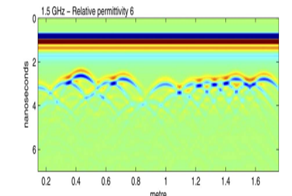
\includegraphics[scale=1]{gambar/bab2/gprmax2.png}
  \caption{Pemodelan sinyal 2D pada gprMax \parencite{Giannopoulos2005}}
  \label{fig:grMax2d}
\end{figure}
\begin{figure} [H] \centering
  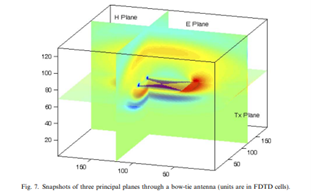
\includegraphics[scale=1]{gambar/bab2/gprmax3.png}
  \caption{Pemodelan sinyal 3D pada gprMax  \parencite{Giannopoulos2005}}
  \label{fig:grMax3d}
\end{figure}

\subsection{Python}
Python merupakan salah satu bahasa pemrograman serbaguna dan tingkat tinggi yang terkenal karena kepopularitasnya. Python berkembang pertama kali pada akhir tahun 1980-an di Belanda, oleh Guido van Rossum. Versi pertama Python yakni 0.9.0, diluncurkan pada tahun 1991, diikuti oleh Python 2.0 pada tahun 2000. Python baru berkembang secara signifikan setelah berjalan 9 tahun lagi. Periode antara tahun 2005 dan 2013 menandai era penting dalam pengembangan Python, peningkatan ini tak lepas dari upaya yang pembuat bahasa python itu sendiri. Python membedakan dirinya dengan menjadi bahasa yang diinterpretasikan, tidak memerlukan programnya untuk dikompilasi menjadi kode mesin. Sebagai gantinya, kode Python diubah menjadi bytecodes, yang kemudian dieksekusi oleh Mesin Virtual Python (PVM) yang terintegrasi dalam interpreter Python\parencite{Harris2023}.

Menekankan aksesibilitas, sintaksnya yang sederhana memudahkan pembacaan dan penggunaan. Meskipun sederhana, Python tetap menjadi bahasa serbaguna yang kuat, menawarkan pengalaman pemrograman yang lebih efisien, terutama bila dibandingkan dengan Java. Kelebihan Python terletak pada dukungannya untuk berbagai pemrograman, termasuk pemrograman terstruktur, imperatif, berorientasi objek, fungsional, dan prosedural. Akan tetapi, ia tidak mendukung pemrograman logika. python memiliki 2 kelebihan antara lain: pertama, python memiliki berbagai konstruksi dan pernyataan bahasa yang kuat untuk representasi dan manipulasi data. Kedua, python memiliki ekosistem yang luas dari paket, pustaka, dan modul pihak ketiga untuk berbagai kebutuhan pemrograman, ditambah dengan perpustakaan standar yang luas yang disertakan dalam setiap rilis Python. Keberagaman ini membuat Python menjadi pilihan populer di bidang seperti analisis data dan pembelajaran mesin, didukung oleh pustaka seperti NumPy, SciPy, Pandas, Matplotlib, dan TensorFlow\parencite{Harris2023}.

Kelebihan python bukan tanpa kekurangan, mengingat interpreter Python membentuk lapisan dasar perangkat lunak, mereka tidak terhindar dari bug perangkat lunak. Masalah dalam interpreter Python cenderung lebih luas dan berpotensi lebih merusak dibandingkan dengan bug aplikasi biasa. Penanganan dan penyelesaian dari bug-bug ini dalam interpreter Python sangat penting untuk memastikan aplikasi Python dapat berjalan seperti yang diharapkan\parencite{Ziyuan2022}.

\subsection{Convolutional Neural Network}
Artificial Neural Network (ANN) merupakan sistem pemrosesan komputasi yang terinspirasi oleh cara sistem saraf biologis otak beroperasi. ANNs terutama terdiri dari sejumlah besar node komputasi yang saling terhubung yang biasa disebut neuron dimana neuron yang bekerja bersama-sama secara terdistribusi untuk belajar secara kolektif dari input agar dapat mengoptimalkan outputnya. Convolutional Neural Network (CNN) memiliki kesamaan dengan ANN yang mana terdiri dari neuron yang mengoptimalkan diri melalui pembelajaran. Setiap neuron akan tetap menerima input dan melakukan operasi dasar dari banyak ANN. Dari vektor gambar mentah input hingga output akhir skor kelas, seluruh jaringan akan tetap mengekspresikan satu fungsi skor perseptif (bobot). Lapisan terakhir akan berisi fungsi kerugian yang terkait dengan kelas, dan semua tips dan trik reguler yang dikembangkan untuk ANNs tradisional masih berlaku\parencite{Keiron2015}.

Bisa dikatakan bahwa CNN adalah model yang cukup baik dalam bidang pemrosesan gambar. CNN dapat memberikan hasil yang baik dalam klasifikasi gambar, pengenalan, segmentasi semantik, dan terjemahan mesin, dan dapat belajar serta mengekstrak fitur gambar secara mandiri. Namun, CNN hanya bisa dioperasikan pada data reguler, seperti gambar dengan ukuran tetap\parencite{Ruyue2020}. Perbedaan yang cukup terlihat antara CNN dan ANN tradisional CNN banyak digunakan dalam bidang pengenalan pola dalam gambar. Hal ini memungkinkan pengguna dalam mengkodekan fitur khusus gambar ke dalam arsitektur, membuat jaringan lebih cocok untuk tugas yang berfokus pada gambar - sekaligus mengurangi parameter yang dibutuhkan dalam mengatur model\parencite{Keiron2015}.

CNN memiliki banyak variasi arsitektur. Namun, komponen dasar CNN bisa dikatakan mirip dimana terdiri dari tiga jenis lapisan, yaitu lapisan konvolusional, pooling, dan fully-connected. Lapisan konvolusional bertujuan untuk belajar representasi fitur dari input\parencite{Jiuxiang2018}.

\begin{figure} [H] \centering
  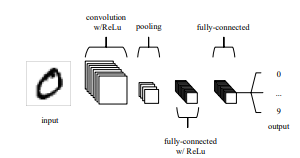
\includegraphics[scale=1]{gambar/bab2/cnn1.png}
  \caption{Arsitektur CNN sederhana \parencite{Keiron2015}}
  \label{fig:CNNArsi}
\end{figure}

Seperti pada ANN, input layer di CNN akan membawa nilai pixel dari gambar\parencite{Keiron2015}. Lapisan konvolusi terbentuk oleh beberapa kernel konvolusi yang digunakan untuk menghitung peta fitur yang berbeda. Setiap neuron dari sebuah peta fitur terhubung dengan sebuah wilayah dari neuron tetangga di lapisan sebelumnya\parencite{Jiuxiang2018}.

\begin{figure} [H] \centering
  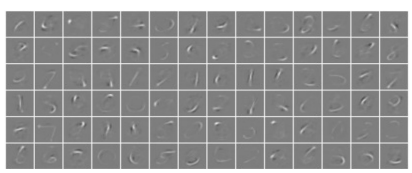
\includegraphics[scale=1]{gambar/bab2/cnn2.png}
  \caption{Aktivasi dari convolutional layer pertama \parencite{Keiron2015}}
  \label{fig:CNNConvo}
\end{figure}

Seperti namanya, lapisan konvolusi memainkan peran penting dalam cara kerja CNN. Parameter lapisan ini berfokus pada penggunaan kernel yang dapat dipelajari. Kernel ini memiliki ukuran kecil dalam dimensi spasial, tetapi menyebar sepanjang seluruh kedalaman input. Saat data mencapai lapisan konvolusi, dilakukan konvolusi setiap filter di seluruh dimensi spasial input untuk menghasilkan peta aktivasi 2D. Peta aktivasi ini dapat divisualisasikan, seperti yang terlihat pada Gambar \ref{fig:CNNConvo}. Saat melalui input, hasil kali skalar dihitung untuk setiap nilai dalam kernel. (Gambar \ref{fig:Blueprint}) Jaringan akan belajar kernel yang 'aktif' ketika mereka melihat fitur tertentu pada posisi spasial tertentu dari input. Ini umumnya dikenal sebagai aktivasi\parencite{Keiron2015}.

\begin{figure} [H] \centering
  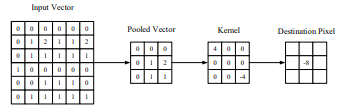
\includegraphics[scale=1]{gambar/bab2/cnn3.png}
  \caption{Representasi visual convolution layer \parencite{Keiron2015}}
  \label{fig:Blueprint}
\end{figure}

Peta aktivasi dimiliki oleh setiap layer konvolusi of yang akan ditumpuk sepanjang dimensi kedalaman membentuk volume output penuh dari lapisan konvolusi\parencite{Keiron2015}.

Lapisan pooling memiliki tujuan untuk mencapai ketidakberubahan pergeseran dengan melakukan pengurangan resolusi peta fitur. Lapisan ini berada di antara dua lapisan konvolusi. Setiap peta fitur dari lapisan pooling tersambung dengan peta fitur yang sesuai dari lapisan konvolusi sebelumnya. Setelah beberapa lapisan konvolusi dan pooling, akan terdapat lapisan fully-connected yang bertujuan untuk menalar dalam tingkat tinggi. Lapisan ini mengambil semua neuron di lapisan sebelumnya dan menghubungkannya ke setiap neuron di lapisan saat ini untuk menghasilkan informasi semantik global\parencite{Jiuxiang2018}.

Fully-connected layer berisi neuron yang terhubung langsung ke neuron di dua lapisan yang berdekatan\parencite{Keiron2015}. Lapisan terakhir dari CNNs adalah lapisan output\parencite{Jiuxiang2018}. Lapisan yang tidak kalah penting adalah lapisan ReLU. Tujuan dari ReLU adalah untuk melakukan peningkatan non-linearitas CNN. Lapisan ReLU sendiri tidak mengubah ukuran dari input dan lapisan ini tidak memiliki parameter. Pada penerapannya, lapisan ini aman untuk digunakan karena lapisan ReLU akan mengatur semua nilai negatif menjadi nol\parencite{Wu2017}.

\subsection{Roboflow}
Roboflow adalah situs web yang memiliki banyak koleksi terhadap berbagai jenis dataset. Website ini juga menyediakan data dalam berbagai pilihan format untuk berbagai model machine learning\parencite{Deepa2023}. Setidaknya, Roboflow memiliki lebih dari 100.000 pengguna yang telah mengumpulkan dan melabeli dataset mereka sendiri untuk kebutuhan kustom mereka. Hal tersebut menyebabkan Roboflow Universe telah banyak digunakan oleh para peneliti untuk digunakan dalam berbagai projek mereka khususnya dalam proyek deteksi objek\parencite{ciaglia2022}.


Sebagai platform computer vision, Roboflow digunakan untuk melatih model karena kemudahan dan kecepatan yang dimiliki dalam membuat model tanpa harus melalui proses pemrograman yang intensif. Roboflow memiliki fitur untuk mempersiapkan data, melatih dan mengembangkan model, serta banyak hal lainnya yang membuatnya menjadikan Roboflow sebagai platform dengan infrastruktur untuk mempercepat proses pembuatan model computer vision. RoboFlow menawarkan rangkaian lengkap alat dan layanan dengan tujuan menyederhanakan dan mempercepat pengembangan dan penerapan model computer vision. Hal ini sangat berguna dalam penggunaan visi komputer pada aplikasi dan proyekb bagi pemrogram dan perusahaan. Fitur dan kemampuan utama RoboFlow meliputi anotasi data dan persiapan untuk memberi label pada video dan gambar, yang keduanya diperlukan untuk mengajarkan model computer vision untuk mengidentifikasi dan menemukan lokasi objek dalam gambar. Dengan menghasilkan varian data asli, RoboFlow menawarkan berbagai strategi augmentasi data yang membantu model machine learning menjadi lebih baik. Model computer vision tersebut nantinya dapat dilatih menggunakan TensorFlow, PyTorch, dan YOLO\parencite{Brucal2023}.

\subsection{YOLO}
You Only Look Once (YOLO) adalah algoritma yang populer dan banyak digunakan. YOLO terkenal dengan karakteristik pendeteksi objeknya. YOLO pertamakali diperkenalkan pada tahun 2015. Dalam beberapa tahun terakhir, YOLO telah mengalami perkembangan dan mencapai versi yang lebih baru seperti YOLO V2, YOLO V3, YOLO V4, YOLO V5, dan seterusnya hingga YOLO V9. Ada beberapa versi revisi terbatas, seperti YOLO-LITE. Ukuran model yang kecil dan kecepatan perhitungan yang cepat merupakan inti dari algoritma deteksi target YOLO. YOLO cepat karena YOLO hanya perlu memasukkan gambar ke dalam jaringan untuk mendapatkan hasil deteksi akhir, sehingga YOLO juga dapat mengukur waktu deteksi video. YOLO secara langsung menggunakan gambar global untuk deteksi, yang dapat mengkodekan informasi global dan mengurangi kesalahan dalam mendeteksi latar belakang sebagai objek. Hasil tes YOLO tidak bagus untuk objek yang jaraknya sangat dekat satu sama lain dan dalam kelompok. Kinerja yang buruk ini disebabkan karena hanya dua kotak dalam grid yang diprediksi dan hanya termasuk dalam kelas objek baru dari kategori yang sama, sehingga muncul rasio aspek yang tidak normal, dan kondisi lain, seperti kemampuan generalisasi yang lemah\parencite{Jiang2022}.

Arsitektur YOLO asli terdiri dari 24 convolution layers, diikuti oleh dua lfully connected layers. YOLO memprediksi lebih dari satu kotak pembatas per sel kisi dimana kotak pembatas yang memiliki Intersection Over Union (IOU) tertinggi dengan ground truth dipilih, yang dikenal sebagai non-maxima suppression. YOLO memiliki dua cacat yaitu satu adalah posisi yang tidak akurat, dan yang lainnya adalah tingkat recall yang lebih rendah dibandingkan dengan metode berdasarkan rekomendasi area\parencite{Jiang2022}. YOLO bukanlah algoritma pertama yang menggunakan Single Shot Detector (SSD) untuk mendeteksi objek. Single Shot Detector (SSD), Deconvolution Single Shot Detector (DSSD), RetinaNet, M2Det, dan RefineDet++ merupakan algoritma yang telah ada sebelum YOLO untuk melakukan pendeteksian objek secara satu tahap. YOLO kelebihan sebagai pendeteksi objek dua tahap dalam hal akurasi dan waktu inferensi. Selain itu, dengan munculnya YOLO, berbagai aplikasi telah menggunakan YOLO untuk mendeteksi dan mengenali objek dalam berbagai konteks dan memiliki performa yang sangat baik dibandingkan dengan pendeteksi objek dua tahap lainnya\parencite{Diwan2022}.

\subsection{Google Colab}
Google Colab adalah environment Jupyter notebook yang berjalan di Google cloud. Colab memungkinkan pengguna lain untuk menggunakan dan berbagi notebook Jupyter tanpa harus mengunduh, menginstal, atau menjalankan apa pun. Jupyter sendiri merupakan adalah proyek open source yang bekerja pada browser yang menyematkan bahasa skrip, pustaka, dan alat untuk visualisasi. Setiap file buku catatan di Jupyter terdiri dari beberapa sel, di mana memiliki outputnya menyatu dalam dokumen termasuk teks, tabel, bagan, dan grafik. Google Colab menyediakan akses langsung ke Google Drive dan GitHub serta layanan cloud gratis dengan GPU dan TPU. Platform perangkat keras yang banyak tersedia di cloud adalah CPU, TPU, dan GPU. CPU gratis untuk Google Colab dilengkapi dengan 2-core Intel Xeon @2.0GHz dan RAM 13 GB serta HDD 33 GB. Masa pakai maksimum VM di Google Colab adalah 12 jam dengan waktu idle 90 menit\parencite{Kimn2021}.

\begin{figure} [H] \centering
  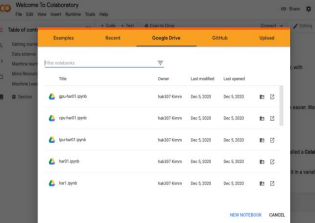
\includegraphics[scale=1]{gambar/bab2/colab.png}
  \caption{Google Colab \parencite{Kimn2021}}
  \label{fig:colab}
\end{figure}

Google Colaboratory adalah platform dapat digunakan untuk melakukan edukasi dan penelitian mengenai machine learning. Colaboratory menyediakan runtime Python 2 dan 3 yang telah dikonfigurasi sebelumnya dengan pustaka machine learning dan AI yang penting, seperti TensorFlow, Matplotlib, dan Keras. Google Colaboratory dapat digunakan secara efektif untuk mempercepat tidak hanya deep learning tetapi juga aplikasi ilmiah berbasis GPU lainnya\parencite{Carneiro2018}.

\subsection{Tensorflow}
Dibuat oleh peneliti yang berasal dari Google, TensorFlow adalah pustaka yang paling populer di antara kebanyakan pustaka lainnya. TensorFlow adalah pustaka perangkat lunak yang fleksibel dan skalabel untuk komputasi numerik menggunakan grafik dataflow. Dengan menggunakan pustaka TensorFlow ini, pengguna mampu memprogram dan melatih neural network serta model machine learning lainnya secara efisien dan menerapkannya ke produksi. Algoritme inti TensorFlow ditulis dalam C++ dan CUDA (Compute Unified Device Architecture) secara optimal. CUDA sendiri merupakan sebuah platform komputasi paralel dan API yang dibuat oleh NVIDIA. CUDA memiliki API yang tersedia dalam beberapa bahasa. Bahasa yang didukung secara resmi oleh TensorFlow adalah JavaScript, C++, Java, Go, dan Swift. TensorFlow juga tersedia untuk lebih banyak bahasa seperti C\# dan Ruby. Akan tetapi, API untuk bahasa pemrograman Python adalah yang paling lengkap dan stabil\parencite{Pang2019}.

TensorFlow adalah platform machine learning menyeluruh yang didukung oleh Google. Pada dasarnya, program TensorFlow terdiri dari dua bagian utama: bagian konstruksi, yang memungkinkan pembuatan model jaringan machine learning atau deep learning, dan bagian eksekusi, yang memungkinkan untuk melatih dan mengevaluasi model jaringan. TensorFlow menyediakan API yang paling banyak digunakan karena kelengkapan dan stabilitasnya yang disajikan dalam bahasa pemrograman Python untuk mencapai kedua bagian tersebut. TensorFlow juga menyediakan pustaka TensorFlow Lite untuk penerapan model jaringan pada perangkat seluler, mikrokontroler, dan perangkat edge. TensorFlow Lite memungkinkan konversi model TensorFlow dasar menjadi versi terkompresi melalui apa yang disebut konverter TensorFlow Lite. Tensorflow sendiri memiliki Keras yang mana merupakan sebuah kerangka deep learning. Keras dibangun di atas TensorFlow versi 2, yang menyediakan API Python untuk memungkinkan pengembang menyederhanakan pembuatan dan eksperimen model jaringan\parencite{Contoli2023}.

\subsection{PyCUDA}
PyCUDA merupakan sebuah API (Application Programming Interface) dari bahasa pemrograman python untuk mengakses kartu grafis NVIDIA menggunakan CUDA. PyCUDA Banyak digunakan sebagai API untuk bahasa pemrograman python adalah karena kode yang ditulis seperti kode python biasa dan penanganan kesalahan juga lebih sederhana daripada bahasa C atau CUDA itu sendiri\parencite{Koprawi2020}. PyCUDA merepresentasikan pendekatan berbasis skrip untuk generasi kode runtime GPU. PyCUDA memberikan kemudahan akses untuk bahasa pemrograman python. Salah satu kemudahan itu ditunjukkan dengan memberikan pengguna akses ke API komputasi paralel milil NVIDIA itu sendiri. Hal tersebut memungkinkan kode CUDA untuk disematkan sebagai string dalam skrip bahasa pemrograman python. String tersebut akan diuraikan oleh pycuda.compilerSourceModule, yang mana akan dikompilasi menggunakan nvcc sebagai driver kompilator CUDA dan terhubung dengan library runtime CUDA. PyCUDA memungkinkan pengguna untuk mengakses GPU NVIDIA menggunakan CUDA dari bahasa pemrograman Python. PyCUDA dirancang untuk pengembang CUDA yang ingin mengintegrasikan kode yang sudah ditulis dalam CUDA dengan Python\parencite{leung2023experience}.

\subsection{NextJS}
Next.JS adalah framework tangguh yang mampu meningkatkan kinerja situs web dan SEO melalui berbagai teknik pengoptimalan. Next.js juga menerapkan Incremental Static Regeneration (ISR) dan mengurangi ukuran beban JavaScript melalui pemisahan kode dan React. Selain kemampuan pengoptimalan dan peningkatan kinerjanya, Next.JS juga menawarkan serangkaian fitur yang memudahkan pengembang dalam membangun dan memelihara situs web mereka. Next.js menyediakan fitur hot reload yang memungkinkan pengembang membuat perubahan pada kode mereka dan melihat hasilnya secara real time tanpa memuat ulang halaman secara manual. Ini bisa menjadi penghemat waktu yang sangat besar bagi pengembang, memungkinkan mereka menguji dan mengulangi kode mereka dengan cepat tanpa perlu pemuatan ulang yang berulang\parencite{Patel2023}. Sebagai salah satu framework yang sering terkenal dan sering digunakan untuk mengembangkan website, Next.js memiliki beberapa kelebihan dalam pengaplikasiannya. Kelebeihan pertama yang dimiliki oleh Next.js adalah didukung dengan kemampuan untuk menggunakan CSS secara langsung pada Next.js. Berbeda dengan penggunaan CSS pada umumnya dimana modul CSS berisi pengaturan CSS untuk semua komponen, pada Next.js terdapat Global CSS yang memungkinkan kode CSS dapat diakses oleh semua komponen\parencite{lazuardy2022}.

\begin{figure} [H] \centering
  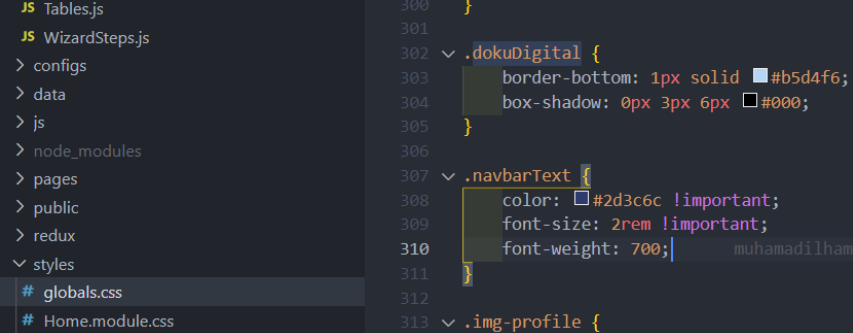
\includegraphics[scale=0.5]{gambar/bab2/builtincss.png}
  \caption{Built-in CSS pada Next.js \parencite{lazuardy2022}}
  \label{fig:builtincss}
\end{figure}

Kelebihan selanjutnya adalah framework Next.js sudah memiliki dukungan mekanisme routing terletak pada folder pages, sehingga tidak memerlukan pustaka tambahan untuk melakukan routing. Routing komponen React cukup dengan menuliskan nama file langsung di folder pages yang disediakan oleh Next.js. Dengan ini, pengguna mampu memasukkan komponen-komponen yang terdapat pada folder komponen ke dalam file routing yang telah disatukan dengan Layout komponen sebagai komponen statis sehingga suatu komponen dapat ditampilkan selama proses pengunggahan\parencite{lazuardy2022}.

\begin{figure} [H] \centering
  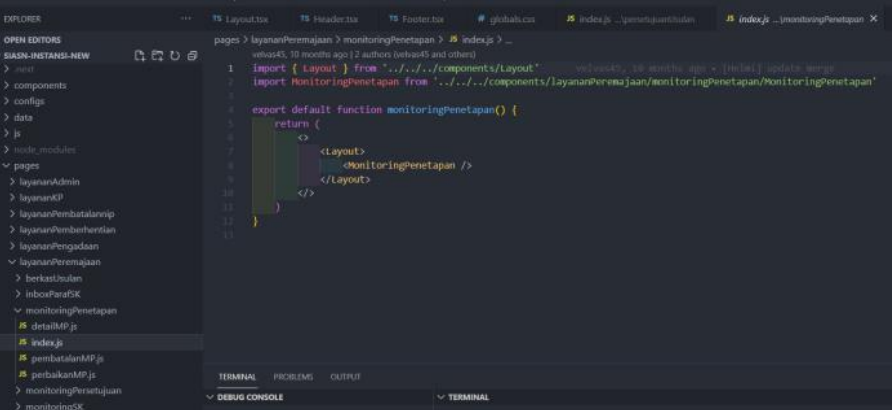
\includegraphics[scale=0.5]{gambar/bab2/routing.png}
  \caption{Routing pada Next.js\parencite{lazuardy2022}}
  \label{fig:routingnextjs}
\end{figure}

Selain itu, kelebihan lain yang dimiliki oleh Next.js adalah Framework Next.js sudah mendukung SSR dalam merender halaman web, sehingga membuat pengguna tidak akan melihat halaman kosong pada pemuatan awal dan mengurangi beban pada browser \parencite{lazuardy2022}.

\begin{figure} [H] \centering
  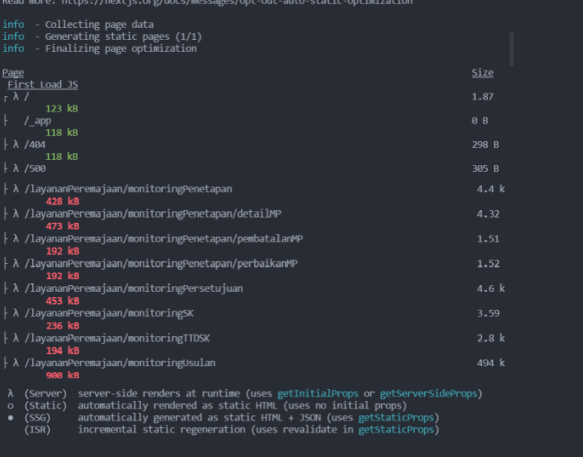
\includegraphics[scale=1]{gambar/bab2/prerender.png}
  \caption{Pre-rendering pada Next.js \parencite{lazuardy2022}}
  \label{fig:prerenderingnextjs}
\end{figure}

Framework Next.js mendukung mekanisme pengambilan data dengan CSR, SSR, SSG, dan ISR yang mana tidak seperti aplikasi React.js biasa yang hanya mendukung pengambilan data dengan CSR. Sehingga mekanisme pengambilan data dapat disesuaikan dengan kebutuhan aplikasi. Menggunakan SSR (server-side rendering) lebih baik untuk SEO (searchengine optimization), daripada CSR (client-side rendering) karena file HTML dirender di sisi server\parencite{lazuardy2022}. Terlepas dari kelebihan ang disebutkan di atas Next.JS mampu melakukan hosting situs web dengan mudah, dengan opsi untuk hosting di platform seperti Vercel dan GitHub Pages. Opsi hosting ini memberi pengembang cara yang nyaman sehingga lebih mudah untuk fokus dalam membangun dan mengoptimalkan situs\parencite{Patel2023}.

\subsection{FastAPI}
FastAPI adalah framework Python berbasis web yang menyediakan lapisan bagi model ML untuk memberikan kinerja tinggi dan mengekspos fungsionalitas model ML sebagai layanan mikro yang tenang. FastAPI terintegrasi dengan baik ke dalam tampilan yang lebih sederhana untuk memprediksi hasil model ML. Aplikasi ini dapat dengan mudah diakses melalui  web browser di Internet. Waktu respon aplikasi FastAPI cukup singkat dibandingkan aplikasi berbasis Flask. Selain itu, biometrik perilaku berpotensi meningkatkan keamanan akun pengguna dan mengurangi jumlah ancaman dan kerentanan tanpa memerlukan perangkat keras tambahan. Studi ini memberikan gambaran komprehensif mengenai penelitian atau upaya yang dilakukan untuk mengintegrasikan model ML dengan FastAPI untuk biometrik perilaku guna memberikan solusi yang lebih cepat dan hemat biaya dibandingkan Flask. Proses pengembangan lebih cepat berkat otomatisasi canggih editor dan pemeriksaan kesalahan otomatis yang disediakan oleh framework \parencite{Bansal2022}.

\subsection{Redis}
Redis adalah penyimpanan struktur data in-memory open-source yang dapat digunakan sebagai database, cache, dan perantara pesan. Redis mendukung berbagai struktur data, termasuk string, hashes, lists, sets, dan sorted sets. Dikenal karena kinerjanya yang luar biasa, Redis dapat menyimpan seluruh kumpulan data di memori, yang secara signifikan mempercepat akses data dibandingkan dengan database berbasis disk. Redis++ memperbaiki manajemen memori dan pengindeksan, yang meningkatkan kinerja dan mengurangi masalah fragmentasi memori dan kehilangan cache\parencite{Zhang2018}. Redis telah diadaptasi untuk menggunakan teknologi RDMA melalui InfiniBand untuk lebih mempercepat kinerja dengan mengurangi latensi jaringan dan pemanfaatan CPU\parencite{Tang2017}. Selain itu, Redis telah diperluas untuk menyertakan fitur keamanan seperti autentikasi dan enkripsi, sehingga lebih cocok untuk aplikasi perusahaan yang memerlukan penanganan data yang aman\parencite{Zaki2015}.

\subsection{Typescript}
Salah satu bahasa pemrograman yang sedang populer untuk mengembangkan aplikasi web adalah TypeScript \parencite{Thu2021}.  TypeScript berkembang sebagai alternatif dari JavaScript yang menerapkan pengecekan tipe statis. Telah banyak perkembangan dan penambahan fitur serta sintax baru dalam bahasa ini. Namun, TypeScript tidak memiliki spesifikasi formal \parencite{Scarsbrook2023}. Perkembangan dari TypeScript diikuti dengan banyaknya pengguna yang menggunakan bahasa ini sebagai bahasa untuk mengembangkan aplikasi website. Akan tetapi, tidak semua fitur yang ada di TypeScript diadopsi oleh pengguna. Pengadopsian TypeScript ini juga mempunyai tantangan \parencite{Thu2021} Beberapa fitur bahasa baru jarang diadopsi oleh proyek-proyek yang ada. Hal ini dikarenakan adopsi fitur baru dalam bahasa TypeScript membutuhkan waktu yang cukup lama. Sebuah proyek dapat memperbarui versi TypeScript tanpa mengubah kode mereka sama sekali, sehingga tanpa mengadopsi fitur baru. Sehingga, mengadopsi fitur baru mungkin memerlukan adopsi versi TypeScript yang baru, tetapi tidak sebaliknya. Hal ini bisa dilihat dari jumlah repositori yang mengadopsi TypeScript terbaru yang berjumlah kurang lebih 1/3 dari mayoritas repositori setelah adanya versi baru dari TypeScript itu sendiri \parencite{Scarsbrook2023}.
